\chapter{Prototype \#1}

This chapter covers the development of my first prototype. I explain the design goals, the creation process, and the brief user testing that was carried out. The chapter closes with a discussion on the significance of the prototype.

\section{Conception}

The first prototype served as an initial experiment for investigating how technology might be used to give an audience new means of participating in a performance. My goal was to develop a simple system that featured a single user `performing' -- creating some sort of stimulating output. Multiple `audience members' would then be given the ability to collectively contribute to this output in some way, illustrating a slight shift from presentational to participatory. Ultimately, testing the prototype with users would allow me to observe how both the performer and audience members responded to these adjustments to their roles. I also hoped to establish a hardware and software framework upon which future prototypes could be easily built.
% It was designed for a colloquium -- to stimulate discussion

While the focus of this thesis is on rock performances, it was decided that recruiting a rock band would not be necessary for this early, small-scale experiment. I felt that a VJ performance would be suitable. VJing is the real-time creation or manipulation of visuals, which are typically projected to accompany music. Thus, the performing user would be controlling projected visuals, and the audience members would be able to manipulate some aspect of them. Having this collective output clearly displayed on one screen would provide the performer and audience members with clear feedback from their inputs and allow for straightforward observations of their interactions.
% Justification for VJ can come from analysis of ethnography; decision that I'll be focusing on visuals and not sound

Some design concepts were inspired by theory introduced in Chapter 2. The system was modelled after the ``core" and ``elaboration" roles outlined by Turino (2008). The performer -- the core role -- would be responsible for keeping the performance on track and have the most influence on the visuals. On the other hand, audience members -- elaboration roles -- would have less responsibility along with a lesser influence. In explaining presentational and participatory performances, Turino also states that it is not uncommon for a performer to shift between the two forms throughout one performance. To reflect this, I chose to include a feature allowing the performer to effectively `mute' input from the audience and take full control of the output.

% Background:
% Auslander, 1999: Communities are formed based on how the audience interacts, with no dependence on the spectacle at hand
% Turino, 2008:
% * Artists can shift between participatory and presentational performance
% * Different roles of different difficult allow for everyone to feel welcome and achieve flow. "Core" and "elaboration" roles cater to advanced and non-advanced performers respectively.
% * Open form: Basic motives repeated over and over. Easy for newcomers to join in. "Security in constancy." Can facilitate flow.
% * Hall: Repetition can increase intensity. Synchronicity comforts people.
% * Wide tuning, loud volumes, and overlapping textures provide a ``cloaking function'' that makes people more comfortable participating
% * Virtuosic solos are not common
% * Some participatory performances are sequential -- everyone gets a turn (e.g. Karaoke)
% Kelly, 2007: Displaying clips and themes from her music videos at a Madonna concert creates feelings of a "shared past" in the audience. (How might we create instead a "shared present"?)
% Small, 1998: Performers dressing in uniform are separating themselves and their responsibilities
% Davidson, 1997:
% * Performance etiquette is usually formed by crowd mentality, following the majority
% * Performers pick up information from the audience's broad and specific behaviours
% * Visuals help audiences read the performer's intentions
% Sexton, 2007: Simple synchronous interactions in sound art projects left users with little to explore, resulting in a "flat" experience
% Jourdain, 1997: We move to music in order to "represent" it. This also amplifies, resonates the musical experience.
% Levitin, 2006:
% * "In every society of which we're aware, music and dance are inseparable." Ancient music was based on rhythm and movement. Combining rhythm and melody bridges our cerebellum and cerebral cortex.
% * Ties between music and movement have only been minimized in the last 100 years
% Kelly, 2007: Technology incorporated into a show can either be addressed as part of the show or hidden and made illusory
% Maynes-Aminzade, 2002:
% * Computer vision: Movement-based control were intuitive, but camera required frequent calibration
% * Beach ball: Using a single beach ball as an input was also intuitive, but it only involved a few people at a time
% * Laser pointers: Gave everyone an individual cursor, but got chaotic once more and more people joined
% * Recommendations: Focus on compelling activity over impressive technology. Not everyone must be sensed as long as they feel involved. The control mechanism should be obvious or the users will give up. Make the activity emotionally engaging. Emphasize cooperation.
% Ulyate, 2001:
% * Design guidelines:
% * * Encourage and reward movement
% * * Feedback should be immediate, obvious, and meaningful in the context of the space
% * * No instruction or thinking should be required
% * * Responsiveness is more important than aesthetics
% * *  Modularity is key
% * Lessons learned:
% * * Full-body movement is most satisfying
% * * Form of the object determines how users interact
% * * A practical system is distributed and scalable
% * * Find balance between freedom and constraint
% * * Users will always find a way to create unwanted outputs
% * * Simple, instant gratification is important for feedback
% Barkhuus, 2008:
% * Inputs based on already-present behaviour lead to intuitive systems
% * Don't focus on employing cutting edge technology
% * Events should not rely on the success of the technology
% * Immediate visual or aural feedback is key
% Tseng, 2012: Being excluded from the interaction did not lessen enjoyment of the show
% Reeves, 2010:
% * "Intra-crowd interaction" is a common phenomena to exploit
% * Many actions "snowball" and overtake crowds; highly visible/audible actions promote this
% * People on the fringes of the crowd interact, but there is latency
% * Every crowd is different; designs should reflect the environment
% Gates, 2006: Technologies should reflect the performer's art and not be a burden on them


\section{Prototyping}

The first step in realizing this initial prototype was deciding on the hardware and software that would be used. Wii video game controllers have an abundance of sensors: they contain eleven digital buttons, an infrared sensor, an accelerometer, and a gyroscope (in the newer Wii Remote Plus models), and all of this data can be sent wirelessly to a receiver via Bluetooth. In addition to these affordances, due to the console's popularity, the Wii controller is also something that many people have already used before. With these considerations, I decided that the Wii controller was a suitable input device for my experiment. For my purposes, the easiest way to process the controllers' data was using a combination of two software packages -- OSCulator\footnote{\url{http://www.osculator.net}} and Max\footnote{\url{http://cycling74.com}}. OSCulator allows for communication between devices and audio or video software using the Open Sound Control (OSC) protocol\footnote{\url{http://opensoundcontrol.org}}. Fortunately, this software is also specifically designed to communicate with the Wii controller. It can display live data from each sensor as well as activate the controller's LEDs and rumble motor. The data can then be sent to Max, a visual programming environment that is especially useful for handling multimedia. Countless objects can be incorporated into a Max program (called a `patcher') to manipulate numbers, audio signals, and video clips. Max is commonly used by musicians and video artists to create highly customized and interactive programs.

\begin{figure}[t]
	\centering

	\includegraphics[height=0.4\textwidth]{osculator_1.png}
	\caption{OSCulator software receiving data from one Wii controller}

	\label{prototyping1.1}
\end{figure}

Syncing the Wii controller with OSCulator was simple, and I was immediately able to view movement and push-button data from my controller (see Figure \ref{prototyping1.1}). Next, I tested the limit of how many Wii controllers would be able to connect to my computer using the current setup. Since my thesis aims to give every member of an audience a new way to participate, this number would ideally be limitless. With Bluetooth technology, unfortunately, one master device (my computer) can only connect to a maximum of seven slave devices (Wii controllers). However, for the purposes of this prototype, I felt that seven controllers would be acceptable. A Max patcher was created to display push-button data from multiple Wii controllers. All seven were synced with no issues, and the program worked as expected (see Figure \ref{prototyping1.2}).

\begin{figure}[t]
	\centering

	\subfloat[Wii controllers]{\includegraphics[height=0.32\textwidth]{wiimotes.jpg}}
	\hspace{0.1cm}
	\subfloat[Max patcher: The LED objects turn yellow when the A button is pressed on their assigned controller]{\includegraphics[height=0.32\textwidth]{multi_wii.png}}
	\caption{Testing simultaneous input from seven Wii controllers}

	\label{prototyping1.2}
\end{figure}

My next task was to create the VJ system. After experimenting with a multitude of video effects objects in Max, I created a basic program. The system is built around two short video loops that can be mixed together and modified. Users can crossfade between the two videos using the controller's Left and Right buttons. The resulting image can be rotated by rotating the controller sideways. Pixelation can be increased or decreased by increasing or decreasing the controller's incline. Finally, holding and releasing the A button enables and disables a motion blur effect. An important part of programming this patcher was mapping controller input to the effects controls. Values had to be carefully scaled and clipped in order for users' movements to translate naturally to the effect they control. I also carefully selected the source video such that the effects of users' actions would be clear; a black and white clip of one person dancing and a colour clip of multiple people dancing seemed to offer sufficient contrast (see Figure \ref{prototyping1.3}). The resultant patcher is pictured in Figure \ref{prototyping1.4}.

\begin{figure}[t]
	\centering

	\subfloat[Black and white]{\includegraphics[height=0.32\textwidth]{vid_1.png}}
	\hspace{0.1cm}
	\subfloat[Colour]{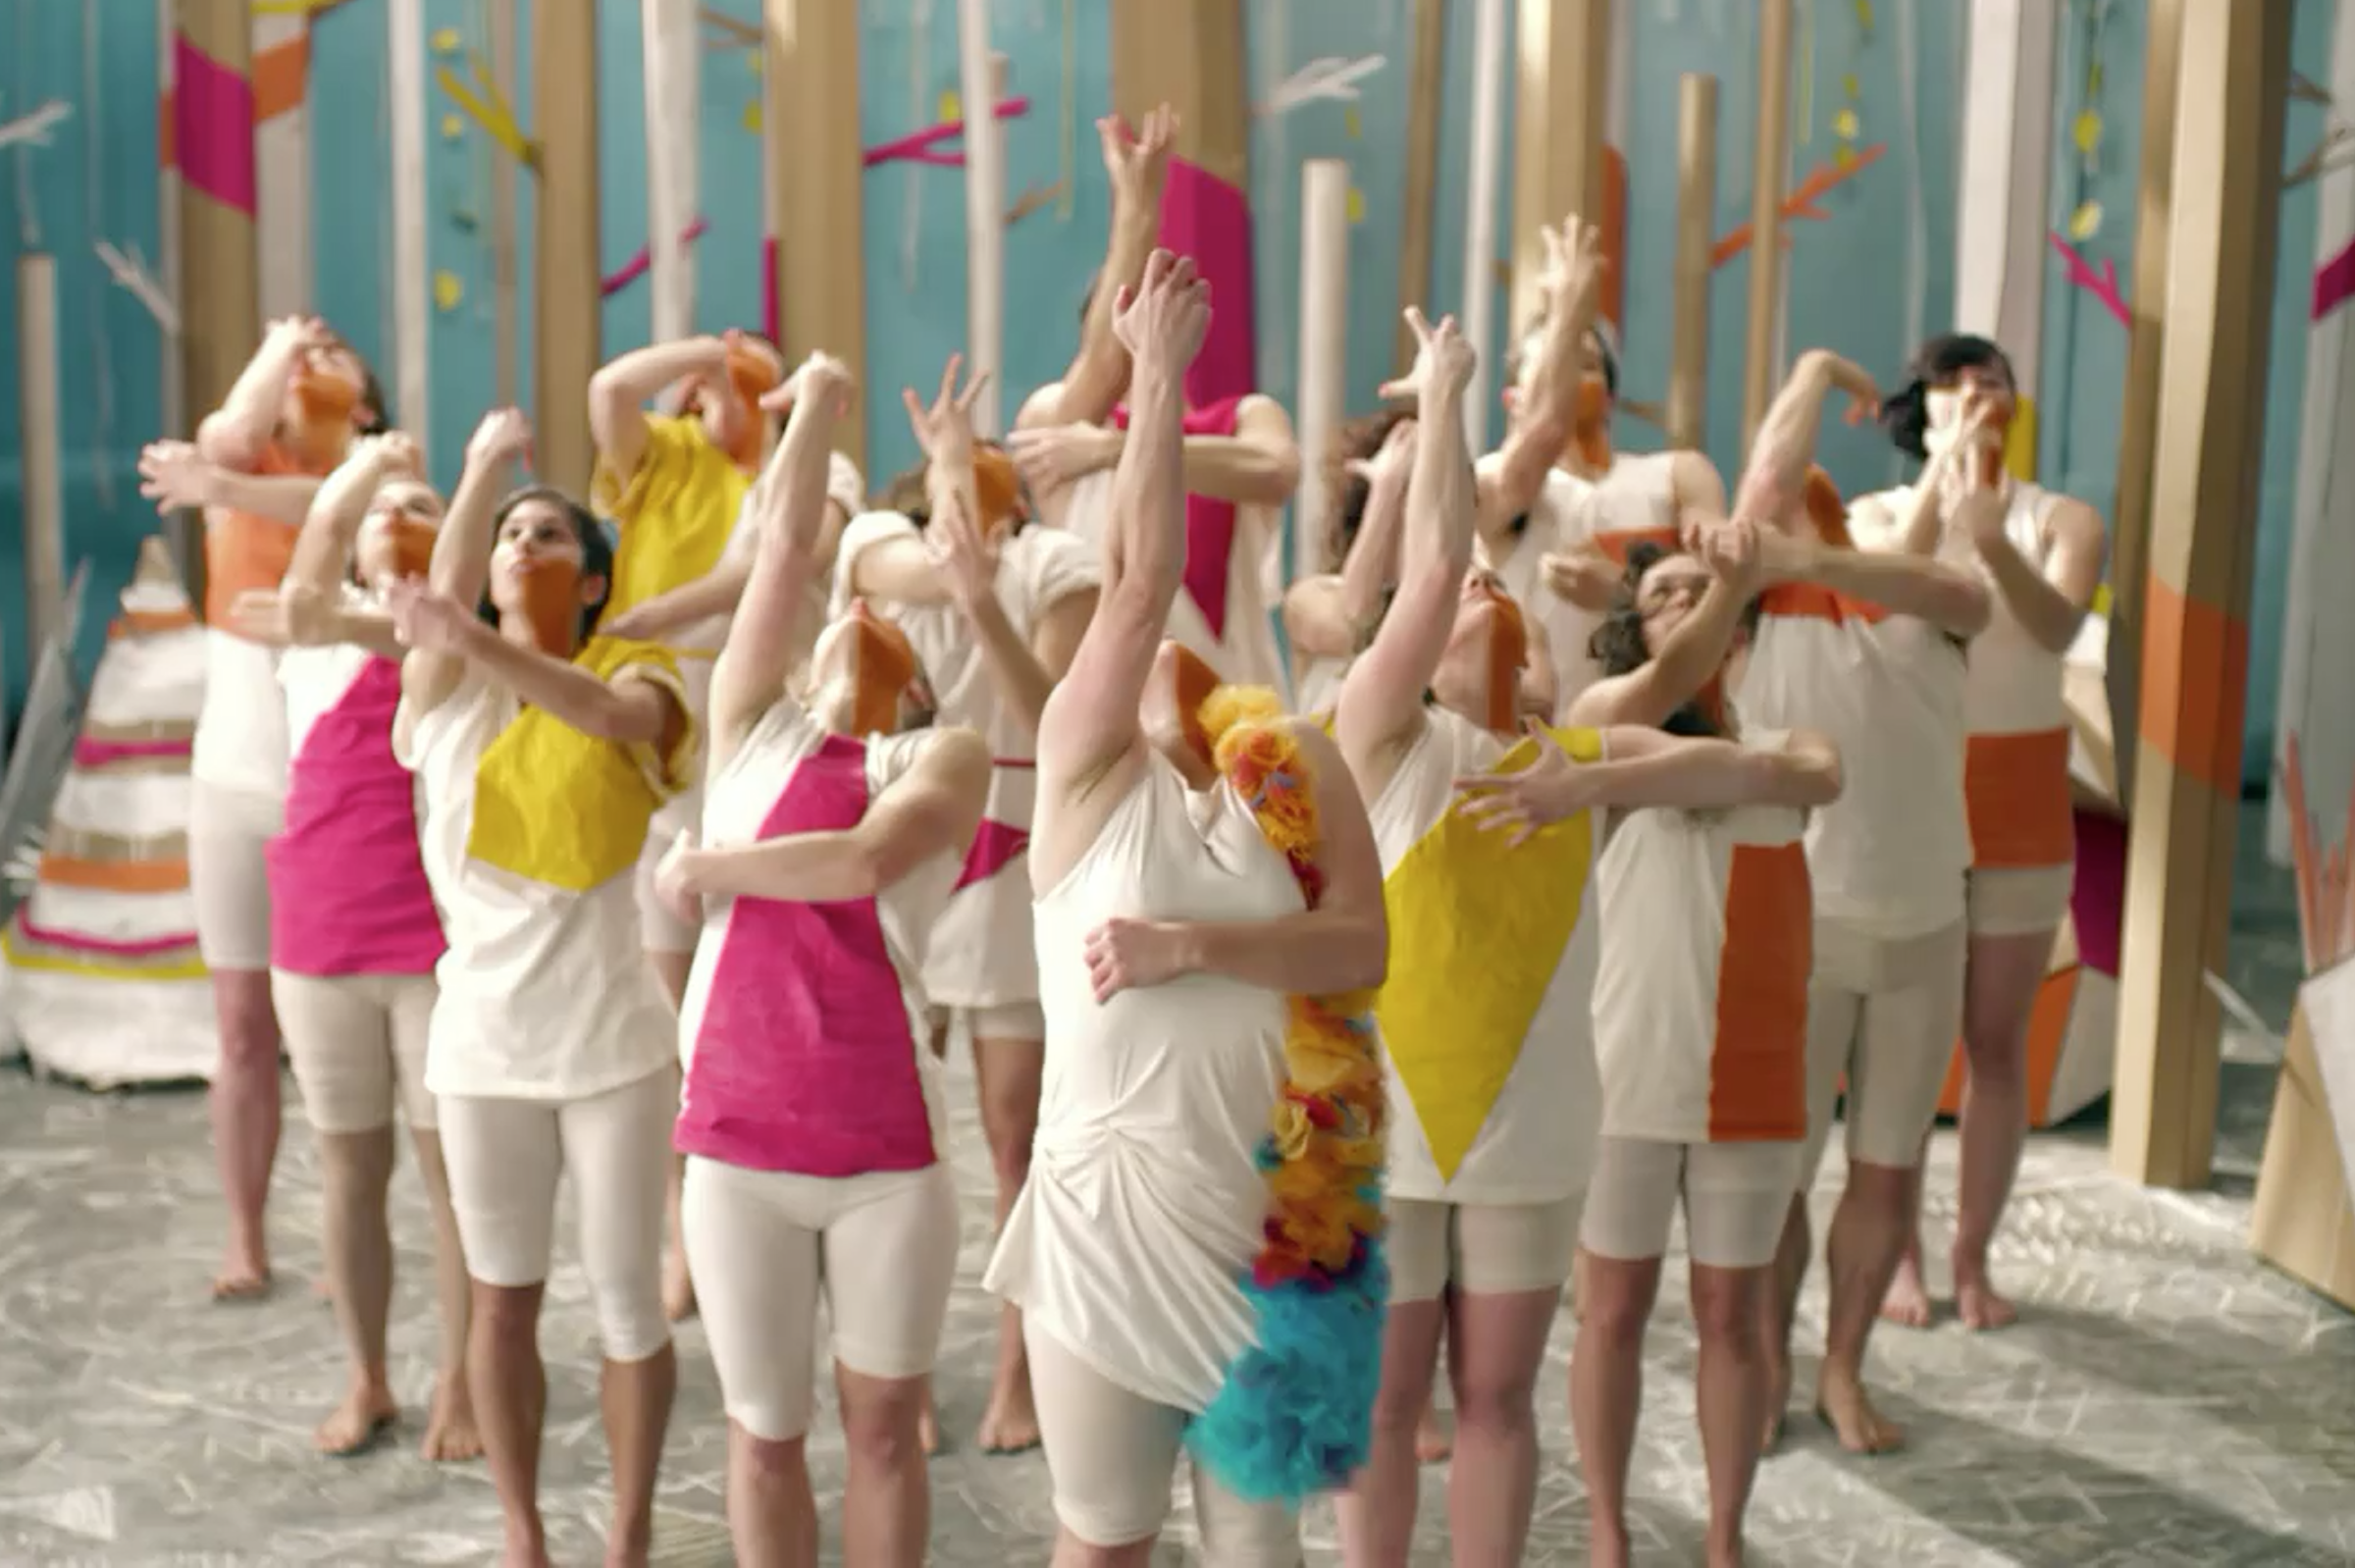
\includegraphics[height=0.32\textwidth]{vid_2.png}}
	\caption{Stills from the two clips used in the prototype}

	\label{prototyping1.3}
\end{figure}

\begin{figure}[t]
	\centering

	\includegraphics[height=0.4\textwidth]{wii_vj.png}
	\caption{Wii controller VJ system}

	\label{prototyping1.4}
\end{figure}

With the details of the performance in place, the next step was selecting which aspect would be controlled by the audience. It seemed most straightforward to give them control over the crossfader effect. This presents audience members with a simple binary decision -- do you want to see more of the black and white video or the colour video? By pressing and holding the Left or Right buttons on their controllers, users can effectively vote on which dominates the screen. In this case, if more people are holding the Left button than the Right, the black and white video will gradually become more prominent than the coloured video. Thus, while the performer retains precise control over multiple combinable effects (rotation, pixelation, motion blur), the collective audience can progressively alter the tone of the visuals. This reflects Turino's (2008) core and elaboration roles, respectively.

The last feature of this VJ system reflects another of Turino's (2008) assertions -- that performers often shift between presentational and participatory performance. In response to this, I provided the performing user with a mute function. By pressing the controller's B button, the performer can disable the audience members' controllers, moving control of the crossfader from the audience to the performer. The B button is essentially an on/off switch for audience participation.

The completed first prototype is illustrated in Figure \ref{prototyping1.5}, in the form of both a diagram and the final Max patcher.
% Make a diagram to illustrate the final product

\begin{figure}[t]
	\centering

	\includegraphics[height=0.4\textwidth]{vj_and_audience.png}
	\caption{Prototype \#1 Max patcher}

	\label{prototyping1.5}
\end{figure}


\section{Testing}
% Explain the details of how participants were recruited, how data was collected, recorded, and processed/analyzed, and the timeline over which this process unfolded

Testing was conducted one time with a small group at a research colloquium. I observed user behaviour and received feedback from attendees. The participants were seven OCADU students. The experiment only lasted a few minutes. I explained the concept and controls. The performer had no problem using his controls to make interesting visual output. One participant led the group in first fading all the way to one video then all the way to the other. Nothing broke, and the group successfully made decisions and carried them collaboratively. The performer's mute button worked.

Context is important; experiments should be run at rock shows or in similar environments. Observers commented on the importance of feedback. They asked if this sort of system should be goal oriented; if not, would the users somehow turn it into a game anyways? They considered the task of representing every individual. Will every single audience member be able to interact? What happens to those who are not included? They referenced `the wave' -- there's a flow, a rhythm; the outcome is greater than the sum of its parts; participants know when it's their turn to input.


\section{Analysis}

% Thoughts:
% * Two buttons: Improving on binary input (cheering, the lighter). Taking audience input from digital towards analog.
% * If we ask the audience to make a decision, will it change throughout the show? (Later: Yes/No vs How; i.e. Prototype 1 vs 3)
% * Mute: When should the audience have control?
% * Goal oriented? Should the users be trying to achieve something? Will they find a way to turn it into a game regardless?
% * What about spectators who are not participants? Tseng et al. indicate those left out can still get enjoyment. Heck, even watching videos of the precedent projects can be exhilarating.
